\documentclass[conference]{IEEEtran}
\usepackage{amsmath,amssymb,graphicx,booktabs,url,xcolor}
\usepackage{tikz}
\usetikzlibrary{arrows.meta,positioning}
\title{Historical Motion Anchors for GNSS Re-entry: A Prospective Multiscenario Study of Accuracy--Delay Tradeoffs}
\author{\IEEEauthorblockN{Internal author-review draft: authors and affiliations unassigned}}
\newcommand{\reviewmark}{\textcolor{red}{\textbf{NOT\_SUBMISSION\_READY: author approval and venue checks pending.}}}
\begin{document}\maketitle
\begin{center}\small\reviewmark\end{center}
\begin{abstract}
Returning GNSS positions can remain biased after an outage. We evaluate a historical motion-anchor admission strategy in a common position filter propagated by FAST-LIO2, separating actual re-entry delay, position error and exposure to artificially displaced observations. All nineteen fixed policies include direct fusion, innovation gates, Huber weighting, seven qualification durations and ablations. Following development, retrospective assessment and a negative joint-gate result on building01, an unchanged multiscenario extension registered new routes and froze complete source, clocks, inputs and caches with verified remote commits before precision access. Every registered route receives natural data and seven fixed GNSS perturbations, without route-specific tuning. The primary post90 biased RMSE for P/Clock2 is street00 2.388/5.848 m; playground00 7.782/8.870 m; building02 8.292/5.483 m. The no-anchor contrast has the same route-dependent directions. street00 is service/cost-qualified but strict NIS is slightly better and faster; playground00 and building02 fail the joint gate, with clean delays of 142 s and a censored event, respectively. Clean recovery, natural cost, all fixed events and stronger simple controls constrain interpretation. The result supports a bounded empirical account of motion anchors and accuracy--delay tradeoffs, not universal superiority or algorithm novelty. Controlled injected-row acceptance and replay-clock bounds are not field fault probabilities or live end-to-end latency.
\end{abstract}
\begin{IEEEkeywords}GNSS recovery, historical anchor, LiDAR--inertial odometry, admission delay, prospective evaluation\end{IEEEkeywords}
\section{Introduction}
A robot may bridge a GNSS outage with LiDAR--inertial odometry (LIO), yet should not necessarily use the first returning receiver position. Persistent position bias can pass a relative-motion check because differences cancel a constant displacement. A historical admitted receiver observation propagated by local motion supplies another constraint, while a stale anchor can veto useful updates. Longer qualification can reduce the error of a finite injected bias by waiting for it to disappear, at a cost to clean re-entry.

The question is whether the inherited P-r03 anchor improves biased-return error relative to the same two-second qualification without an anchor, and relative to complete strong simple alternatives, under explicit clean-delay and natural-cost conditions. All parameters remain unchanged. We distinguish numerical improvement over Clock2 or a no-anchor ablation from satisfying the full service/cost gate, and report any disagreement.

This study adds prospectively registered street00 and playground00, with building02 included on technical availability before any new precision result. building00 and parking00 are seen evidence. building01 was prospective in S8, but its natural-cost failure was known before this extension; it is not relabeled unseen. The contribution is a complete, reproducible empirical comparison and its applicability limits. FAST-LIO2 and KF-GINS retain their attribution; no new full navigation filter or integrity guarantee is claimed.
\section{Related Work}
FAST-LIO2 estimates local motion through direct LiDAR--inertial estimation~\cite{fastlio2}. We use the fixed i2Nav AT128/ADIS adaptation, rather than modifying its point-cloud estimator. KF-GINS implements a separate 21-dimensional GNSS/INS error-state filter~\cite{kfgins}; its posterior is not fed repeatedly into the three-dimensional filter studied here. Huber's robust estimation~\cite{huber} motivates a standard covariance-weighting comparator; innovation gating provides another simple selection rule.

WinTA-GIL~\cite{winta} uses windowed trajectory matching and motion/quality-triggered heading refinement, feeding optimized heading into an EKF. Our implementation keeps its initial local-to-NED alignment fixed and manages receiver-position admission. This scope difference is not a novelty proof: motion windows and recovery-triggered consistency already have precedent.

Dual-ACKF~\cite{dual} combines an explicit GNSS bias state, innovation-based covariance adaptation, robust updates, and recovery protection. Our availability-based control uses the same outer position KF as every other policy; it is not a reproduction of the full Dual-ACKF system. Neither Dual-ACKF nor WinTA-GIL was executed in this benchmark, and their published accuracy is not inserted into our comparison tables. Their mechanisms constrain what this study can claim as original.

\section{Common Filter and Existing Recovery Policy}
\subsection{Shared Estimator}
\begin{figure}[t]
\centering
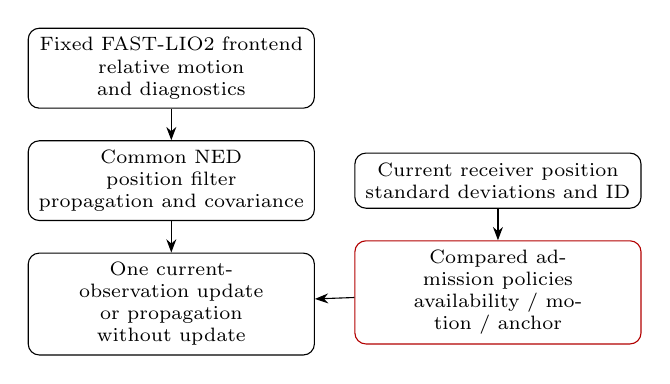
\begin{tikzpicture}[node distance=4mm,every node/.style={draw,rounded corners,font=\scriptsize,align=center,text width=34mm,minimum height=7mm},>=Stealth]
\node (lio) {Fixed FAST-LIO2 frontend\\relative motion and diagnostics};
\node[below=of lio] (prop) {Common NED position filter\\propagation and covariance};
\node[right=5mm of prop] (gnss) {Current receiver position\\standard deviations and ID};
\node[below=of gnss,draw=red!70!black] (manage) {Compared admission policies\\availability / motion / anchor};
\node[below=of prop] (update) {One current-observation update\\or propagation without update};
\draw[->] (lio)--(prop);\draw[->] (prop)--(update);\draw[->] (gnss)--(manage);\draw[->] (manage)--(update);
\end{tikzpicture}

\caption{Executed framework. Only the admission policy varies. Reference states initialize the declared common condition and support offline evaluation; they never enter the manager. KF-GINS remains an independent comparator.}
\label{fig:framework}
\end{figure}
The state is position $p\in\mathbb{R}^{3}$ in NED, with a common initial alignment $A$. For LIO displacement $\Delta\ell_k$,
\begin{align}
 p_k^-&=p_{k-1}^++A\Delta\ell_k,\\
 P_k^-&=P_{k-1}^++\operatorname{diag}(1,1,4)q_k,\\
 q_k&=0.001\Delta t+0.001\|\Delta\ell_k\|.
\end{align}
The coefficients have units $\mathrm{m^2/s}$ and $\mathrm{m^2/m}$. The antenna observation is $z_k=p_k+R_{NB,k}b+v_k$, with FRD lever arm $b=[0,-0.07,-0.365]^\top$ m. Receiver NED standard deviations are floored at $[1,1,2]$ m before squaring to form covariance $R_k$. For an admitted observation,
\begin{align}
 r_k&=z_k-p_k^--R_{NB,k}b,\\
 K_k&=P_k^-(P_k^-+\bar R_k)^{-1},\\
 p_k^+&=p_k^-+K_kr_k,
\end{align}
with Joseph covariance update and policy-inflated $\bar R_k$. Every original receiver ID is consumed once, including rejected observations. Monitoring differences and historical anchors are not independent position measurements.

\subsection{Motion and Historical Anchor}
With receiver position $z$ and independent LIO antenna position $a$, a five-second window checks
\begin{align}
 d_{ik}&=(z_k-z_i)-(a_k-a_i),\\
 s_{ik}&=d_{ik,xy}^{\top}(R_{k,xy}+R_{i,xy}+q_{ik}I)^{-1}d_{ik,xy}.
\end{align}
The existing P-r03 policy requires an engineering score at most four for two seconds when a motion qualification applies. This score is not a calibrated chi-square test. Gaps greater than 1.5 s clear the monitoring window. An availability shadow policy isolates an anomaly or a GNSS gap greater than two seconds, with a two-second minimum wait and a covariance multiplier initially 15, relaxing over 15 s.

A historical anchor stores the latest raw GNSS observation that was admitted in NORMAL state with valid local diagnostics, acceptable motion score and nominal innovation, continuously qualified for five seconds. During outage recovery it compares
\begin{equation}
 e_k=z_k-\{z_a+(a_k-a_a)\}
\end{equation}
against receiver covariance plus accumulated process covariance. Its horizontal score limit is four. Only an actual GNSS gap activates this anchor check; isolation freezes anchor promotion. Invalid local evidence falls back to the mature availability policy and is logged as unresolved, not as proof of sensor correctness. The two cached interpolation endpoints must have at least 100 effective points and mean absolute plane residual at most 0.2 m for local health eligibility.

This policy cannot distinguish all LIO drift from GNSS bias. A stale or biased anchor can veto useful GNSS; fallback can admit injected observations. There is no bias-state estimation, optimized heading update, or integrity guarantee. The fixed implementation is inherited from R1 rather than revised to fit the R2 results.



\section{Data and Prospectively Frozen Protocol}
\subsection{Route Roles and Common Inputs}
The i2Nav-Robot dataset~\cite{i2nav} supplies AT128 LiDAR, ADIS16465 angle/velocity increments and F9P single-point receiver positions. Upstream versions and the existing isolated Noetic frontend remain fixed. All five originals per new route are read-only; each bag matches its official SHA-256. Text digests are local identities. Extras and failed engineering attempts are retained. street00/playground00 are the priority new scenes; building02 is included before opening precision because its actual originals and complete cache passed technical checks, despite a retained download-sidecar file.

Standard/custom IMU, F9P text and ROS headers establish each clock independently: playground00 is GPS week 2363, street00/building02 week 2364, with 18-s GPS--UTC difference. Text uses seconds of week. Custom IMU increments match text; they are not rates multiplied by dt again. One predetermined full 1$\times$ replay per route uses the same AT128/ADIS pipeline. At most two isolated technical replays run concurrently; no cache is chosen by accuracy and no deployment timing is inferred. Public metadata pages also display published standard-baseline performance; it was not used to select parameters/routes or inserted as our run results. The prospective guarantee is first local strategy-error access after freeze, rather than ignorance of public literature.

All policies on a route use identical LIO cache, GNSS observations, initialization, Q/R and lever arm. S9 selects one original reference state at the earliest timestamp covered by IMU, valid causal GNSS and the primary LIO cache. Selection scans timestamps, not positioning error, and the same row initializes every policy. Playground/building02 references begin before recorded sensors; this explicit pre-freeze interface rule avoids initializing outside coverage. street00 has one duplicate first reference timestamp; stable first-row retention is fixed before precision, with raw rows unchanged. Remaining reference states are used only offline. Local-to-NED alignment is fixed, without method-specific trajectory fitting or claimed absolute origin recovery.

The new routes use navigation-grade GNSS/INS reference with OEM719 information; prior building01/parking00 use MM/INS with shared AT128 map matching. Neither reference construction establishes independence from every sensing/error source. The common reference/ADIS/primary-LIO timestamp interval, rather than the longer published reference duration, defines the full expected evaluation grid. The prior unresolved 3.6013-m RMS frontend repeat difference remains a limitation, not a reason to select a favorable cache.

\subsection{Fixed Controls, Events and Endpoints}
B2 is LIO-only; B3 direct fusion; B4 NIS100; B5 Huber2.5; B6 availability-based protected recovery. Strict NIS11.3449/16.2662/30 retain their screened parameters. Clock2/5/10/15/30/60/90 disable motion/anchor veto while retaining availability and covariance protection. P-no-anchor and P-no-decay remove those components; P-no-motion equals B6 and time-only equals Clock2. These nineteen names include aliases, not nineteen original algorithms. Clock numbers denote qualification durations: monitoring windows and unresolved local-health fallback affect actual admission. Clock2 has the same two-second qualification as P, but actual event delays are measured rather than assumed equal.

At 150/450/750-s offsets from common initialization with N/E/NE directions, seven categories retain three events each:3-m single jump,10-m clustered jumps,30/60-s deletions with unchanged return,30-s deletions then3/10-m biases held90s, and a10-m ramp. Natural data is the eighth case. Complete 10/30/60/90/180-s post-return windows are checked against common support before the collective freeze. No event or route is selected by method error. Complete scientific source/tests, nineteen parameters, calibration, runtime/binary/cache, five raw identities and metric definitions are committed, pushed and exactly remotely verified for all included routes before the first new matrix opens.

The primary biased error is the equal-weight mean of three post90 horizontal RMSEs after30-s deletion and90-s10-m bias. All windows and whole-route evaluation use a full 10-Hz expected grid, retaining missing/partial/censored status rather than successful intersections. Actual $t_{admit}$ is the first logged \texttt{accepted=true} KF update after the first physically present returning measurement; admission is censored at 180 s. Clean measurement-time delay must be at most 15 s, inclusive with $10^{-8}$-s tolerance. Conservative cache-availability bounds and5/10/30/60/90-s sensitivity budgets remain separate. Neither cached clock measures field end-to-end delay.

Joint qualification also requires full coverage and natural RMSE no greater than the best B4/B5/B6 natural error plus $\max(2\%,0.05\,\mathrm{m})$. This gate never removes unqualified controls from raw tables. Injected accepted/exposed IDs measure controlled exposure, not field error probability; displacement can cancel original receiver error. P95/Max, all categories, extended windows and all individual events remain in the evidence. Cross-route aggregates weight each registered route equally and do not discard unfavorable signs.

\section{Results}
\begin{table*}[t]\centering\small
\caption{All nineteen frozen policies: biased-return 90-s horizontal RMSE (m), equal-weight mean over all three fixed events. Building00/parking00 are seen; building01 was prospective in S8 and already seen before S9. The other columns are S9 prospective routes. No policy or unfavorable route is removed. Full natural, latency, exposure and extended-window records accompany the paper.}\label{tab:allroutes}
\begin{tabular}{lrrrrrr}\toprule
Policy & Building00 & Parking00 & Building01 & Street00 & Playground00 & Building02 \\\midrule
LIO only & 1.773 & 2.226 & 1.325 & 3.062 & 6.194 & 10.052 \\
Direct fusion & 8.371 & 7.015 & 4.030 & 8.782 & 9.896 & 7.301 \\
NIS100 & 8.371 & 3.091 & 4.030 & 8.665 & 11.646 & 6.175 \\
Huber2.5 & 7.645 & 6.426 & 3.782 & 8.208 & 9.655 & 6.401 \\
Availability B6 & 5.780 & 4.478 & 3.182 & 6.145 & 9.097 & 5.603 \\
NIS11.3449 & 3.653 & 2.164 & 2.998 & 2.388 & 8.968 & 12.768 \\
NIS16.2662 & 3.700 & 2.128 & 2.472 & 2.388 & 7.063 & 12.768 \\
NIS30 & 3.908 & 2.023 & 3.170 & 2.388 & 7.293 & 12.768 \\
Clock2 & 5.558 & 4.395 & 3.160 & 5.848 & 8.870 & 5.483 \\
Clock5 & 5.490 & 4.374 & 3.157 & 5.812 & 8.836 & 5.508 \\
Clock10 & 5.361 & 4.116 & 3.140 & 5.691 & 8.767 & 5.550 \\
Clock15 & 4.899 & 3.758 & 2.902 & 5.145 & 8.701 & 5.579 \\
Clock30 & 4.427 & 3.403 & 2.844 & 4.493 & 8.663 & 5.761 \\
Clock60 & 2.838 & 2.521 & 2.368 & 2.762 & 9.008 & 6.356 \\
Clock90 & 2.510 & 2.298 & 2.362 & 2.388 & 9.166 & 6.830 \\
P-r03 & 3.022 & 2.290 & 2.378 & 2.388 & 7.782 & 8.292 \\
P-no-motion & 5.780 & 4.478 & 3.182 & 6.145 & 9.097 & 5.603 \\
P-no-anchor & 5.489 & 4.395 & 3.172 & 5.848 & 8.895 & 5.480 \\
P-no-decay & 3.059 & 2.259 & 2.388 & 2.388 & 8.158 & 8.605 \\
\bottomrule\end{tabular}\end{table*}
\begin{table*}[t]\centering\small
\caption{Prespecified S9 mechanism contrasts, strong simple controls and strongest jointly qualified control per route. Natural is whole-route horizontal RMSE; Clean is maximum actual clean GNSS measurement-time admission delay (s). Bias90/180 are matched macro RMSE (m). Exposure is accepted/exposed injected rows. Q requires clean delay at most15 s, frozen natural-cost cap and full coverage. Qualification durations are not unconditional waiting times; all nineteen complete results are retained.}\label{tab:primary}
\begin{tabular}{llrrrrrc}\toprule
Route & Policy & Natural & Clean & Bias90 & Bias180 & Exposure & Q\\\midrule
street00 & P-r03 & 1.673 & 7.000 & 2.388 & 2.341 & 0/270 & yes \\
street00 & Clock2 & 1.673 & 7.000 & 5.848 & 5.719 & 239/270 & yes \\
street00 & P-no-anchor & 1.673 & 7.000 & 5.848 & 5.795 & 239/270 & yes \\
street00 & NIS30 & 1.656 & 0.000 & 2.388 & 2.151 & 0/270 & yes \\
street00 & Huber2.5 & 1.673 & 0.000 & 8.208 & 6.720 & 270/270 & yes \\
street00 & Clock90 & 1.673 & 95.000 & 2.388 & 2.058 & 0/270 & no \\
street00 & NIS11.3449 & 1.656 & 0.000 & 2.388 & 2.253 & 0/270 & yes \\
playground00 & P-r03 & 5.935 & 142.000 & 7.782 & 8.210 & 26/270 & no \\
playground00 & Clock2 & 5.935 & 7.000 & 8.870 & 8.965 & 239/270 & no \\
playground00 & P-no-anchor & 5.935 & 7.000 & 8.895 & 9.074 & 239/270 & no \\
playground00 & NIS30 & 3.142 & C180 & 7.293 & 7.872 & 85/270 & no \\
playground00 & Huber2.5 & 4.112 & 0.000 & 9.655 & 8.426 & 270/270 & no \\
playground00 & Clock90 & 5.935 & 95.000 & 9.166 & 7.952 & 0/270 & no \\
playground00 & Direct fusion & 3.142 & 0.000 & 9.896 & 7.700 & 270/270 & yes \\
building02 & P-r03 & 6.498 & C180 & 8.292 & 8.907 & 22/270 & no \\
building02 & Clock2 & 6.498 & 7.000 & 5.483 & 5.416 & 231/270 & no \\
building02 & P-no-anchor & 6.498 & 7.000 & 5.480 & 5.514 & 231/270 & no \\
building02 & NIS30 & 3.384 & 65.000 & 12.768 & 13.382 & 0/270 & no \\
building02 & Huber2.5 & 4.043 & 0.000 & 6.401 & 5.494 & 270/270 & no \\
building02 & Clock90 & 6.498 & 95.000 & 6.830 & 6.535 & 0/270 & no \\
building02 & NIS100 & 3.384 & 0.000 & 6.175 & 4.715 & 27/270 & yes \\
\bottomrule\end{tabular}\end{table*}

\begin{figure*}[t]\centering
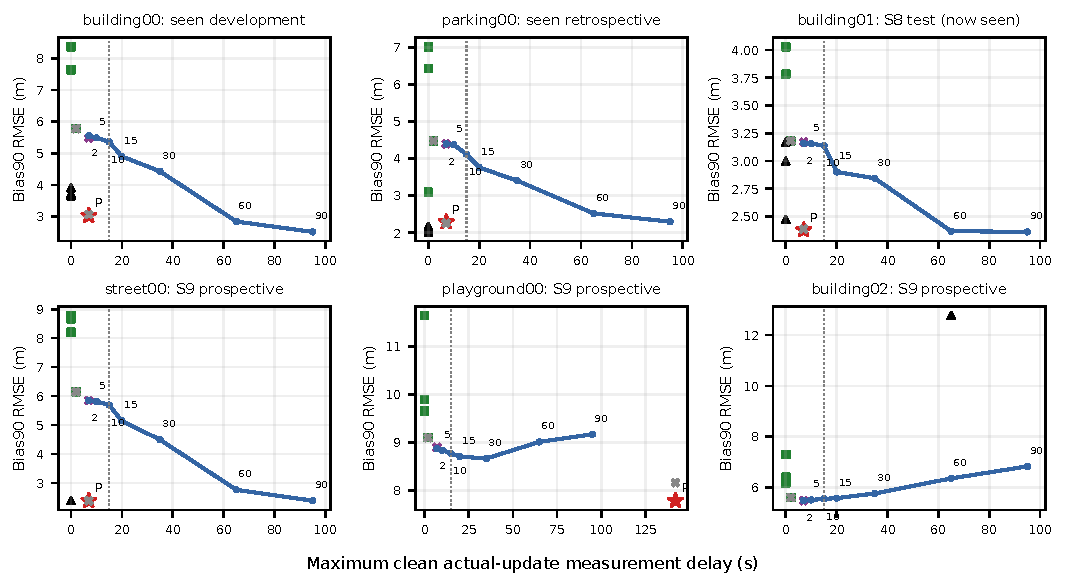
\includegraphics[width=\textwidth]{figures/multiroute_tradeoff.pdf}
\caption{Every fixed route and finite-delay policy. Clock labels are qualification durations; dotted line marks15-s clean measurement-time budget. Red stars are P, crosses ablations, triangles strict NIS, squares established baselines. Each panel has its own vertical scale. Censored LIO-only remains in the table and exported points. Lower raw error outside service/cost gates is retained.}
\label{fig:tradeoff}\end{figure*}
\subsection{Complete New-Route Comparison}
street00: P gives natural RMSE 1.673 m against the 1.706-m cap, maximum clean delay 7.0 s, and biased post90/post180 RMSE 2.388/2.341 m. Clock2 gives 5.848 m, no-anchor 5.848 m, NIS30 2.388 m, Huber2.5 8.208 m and Clock90 2.388 m. P passes the joint qualification. The strongest joint-qualified alternative is NIS0, with 2.388-m biased error, 1.656-m natural error and 0.0-s clean delay.

playground00: P gives natural RMSE 5.935 m against the 3.205-m cap, maximum clean delay 142.0 s, and biased post90/post180 RMSE 7.782/8.210 m. Clock2 gives 8.870 m, no-anchor 8.895 m, NIS30 7.293 m, Huber2.5 9.655 m and Clock90 9.166 m. P fails the joint qualification. The strongest joint-qualified alternative is B3, with 9.896-m biased error, 3.142-m natural error and 0.0-s clean delay.

building02: P gives natural RMSE 6.498 m against the 3.452-m cap, maximum clean delay censored s, and biased post90/post180 RMSE 8.292/8.907 m. Clock2 gives 5.483 m, no-anchor 5.480 m, NIS30 12.768 m, Huber2.5 6.401 m and Clock90 6.830 m. P fails the joint qualification. The strongest joint-qualified alternative is B4, with 6.175-m biased error, 3.384-m natural error and 0.0-s clean delay.

Independent native KF-GINS with the unchanged STD-scale 2 transfer has natural horizontal RMSE street00 1.007 m (coverage 1.000000); playground00 1.115 m (coverage 0.999925); building02 1.669 m (coverage 1.000000). These real GNSS/INS results are retained even when they are stronger than the LIO-propagated policies; no new-route noise search or KF posterior injection is performed, and this is not a P-gain denominator.

The complete matrix runs all 19 policies in all 8 conditions per new route. An independent checker that does not import the evaluator recomputes whole-route/window RMSE, actual accepted admission, availability bounds and injected exposure. Original 64 tests, 9 R2 metric tests and three sets of 9 S9 role/config/numeric/metric tests pass. All whole-grid coverage, missing records and command exits accompany the tables; technical failures are retained. No new-route parameter or algorithm revision is performed.

\subsection{Anchor Attribution and Adverse Events}
\begin{table}[t]\centering\scriptsize
\caption{All three registered biased events on every S9 route. Horizontal post90 RMSE (m); P admission is its actual biased-return update delay, separate from clean delay. Exposure is P accepted/exposed injected rows. No favorable event subset.}\label{tab:events}
\begin{tabular}{lrrrrr}\toprule
Route/direction & P & Clock2 & No-anchor & P delay & Exposure\\\midrule
street00/N & 0.797 & 5.370 & 5.370 & 97 & 0/90 \\
street00/E & 1.660 & 3.754 & 3.754 & 97 & 0/90 \\
street00/NE & 4.707 & 8.419 & 8.419 & C180 & 0/90 \\
playground00/N & 3.118 & 6.108 & 6.108 & C180 & 0/90 \\
playground00/E & 5.703 & 9.548 & 9.548 & 64 & 26/90 \\
playground00/NE & 14.526 & 10.954 & 11.028 & C180 & 0/90 \\
building02/N & 3.185 & 3.729 & 3.729 & C180 & 0/90 \\
building02/E & 9.828 & 4.803 & 4.803 & 68 & 22/90 \\
building02/NE & 11.863 & 7.917 & 7.907 & C180 & 0/90 \\
\bottomrule\end{tabular}\end{table}
Table~\ref{tab:events} reports every prespecified primary event, including delays inside the biased interval and after it. A lower P macro error against Clock2 cannot by itself identify the anchor contribution: no-anchor holds the remaining manager fixed, while no-decay changes weighting. Full per-event paired differences and no-decay results constrain attribution. Same clean qualification does not guarantee equal delayed admissions during biased recovery. Long waiting can obtain lower raw error at a slower clean return; its local-health fallback may also admit earlier unresolved observations. Complete accepted-row logs preserve these cases rather than declaring the duration a guaranteed quarantine.

The new-route descriptive signs are: The primary post90 biased RMSE for P/Clock2 is street00 2.388/5.848 m; playground00 7.782/8.870 m; building02 8.292/5.483 m. The no-anchor contrast has the same route-dependent directions. street00 is service/cost-qualified but strict NIS is slightly better and faster; playground00 and building02 fail the joint gate, with clean delays of 142 s and a censored event, respectively. Table~\ref{tab:allroutes} includes strict NIS, Huber, long waits and every ablation irrespective of qualification; the evidence package reports paired natural-cost differences and all event signs, not only winning comparisons. A small mean advantage with opposing individual events is treated as a conditional effect, not universal rejection of persistent bias. If P fails the natural or clean gate, raw biased improvement is explicitly separated from compliant service gain.

\subsection{Preserved Earlier Counterevidence}
On building01, P clean admission is 7 s and bias90 error 2.378 m versus eligible B3/B4 at 4.030 m, but natural 5.273 m exceeds the frozen 5.055-m cap. Its biased event admissions are 97/7/7 s; accepted injections are 0/83/83 of 90 each, and the second event is worse than B3/B4. Clock90 raw error 2.362 m is lower than P, despite 95-s maximum clean delay; its second biased event falls back at 17 s. No-decay has lower natural and180-s error. These S8 failures remain unchanged.

On seen parking00, NIS30 is faster and lower in bias90 than P (0s/2.023m versus7s/2.290m). On seen building00, P bias90 is 3.022 m versus Clock10 at 5.361 m, but Clock90 reaches 2.510 m with 95-s clean delay. Its second frontend cache is retained sensitivity, not another route. R1's \texttt{NO\_ADDITIONAL\_GAIN} remains intact. The independent S8 native KF-GINS fixed-configuration transfer gives 17.10-m natural error; it is neither the best possible KF-GINS configuration nor a denominator for P improvement, and its posterior is not injected into P.

\section{Discussion and Applicability}
Persistent receiver displacement cancels in short relative-motion differences; the historical anchor can provide longer memory, while carrying older GNSS error and LIO drift. The observed comparisons apply to the registered finite artificial biases, common controlled initial states and these route overlaps. Accepted injections can partly cancel receiver error, so exposure and position error are distinct endpoints. Anchor staleness, unresolved local-health fallback and nonuniform no-decay effects remain failure mechanisms. Actual delayed updates, clean service and natural-route cost must be assessed jointly.

The extension adds scene diversity without new-route tuning. It remains a fixed descriptive study: within-route events are correlated, reference systems differ, and three new routes do not establish a population-wide effect or calibrated integrity. Known initialization and fixed alignment restrict transfer. Shared GNSS error sources and the earlier frontend repeat discrepancy remain unresolved. Native mapping timing excludes preprocessing/publication/wait; Python cache replay excludes frontend/transport. No result establishes field realtime admission or actual multipath identification.

\section{Conclusion}
Historical motion anchors can alter the error--admission tradeoff, but their value depends on the route, event and application gates. This complete prospectively frozen extension reports all 19 unchanged policies, same-qualification/no-anchor contrasts, stronger simple alternatives and all adverse events. Numerical biased-return changes are separated from satisfying clean 15-s service, natural-cost and coverage requirements. The evidence supports a bounded empirical review manuscript; it does not automatically establish novelty, compliant universal superiority or readiness for formal submission.

\section*{Reproducibility and Acknowledgments}
S9 source/configuration/input/cache hashes, collective freeze and verified remote receipts, all route/event tables, vector figures and independent checks are retained on the separate authorized branch. R1/R2/S8 sources, failures and paper versions remain unchanged. Raw bags/runtime/full numeric caches remain local; Git is a partial evidence backup. The current PDF is for author review, with no assigned authors/affiliations/funding. Exact venue template variant, anonymity, cutoff/timezone and applicable AI rules require human confirmation; no login, payment, copyright agreement or formal submission is performed.

OpenAI Codex (GPT-6) assisted orchestration, evaluation/plot code, evidence organization and drafting of the abstract and all text sections. Numerical figures derive from retained real runs. Human authors must verify interpretation, code, references and wording before adoption; disclosure does not replace author responsibility or venue-specific rules.
\bibliographystyle{IEEEtran}\bibliography{references}
\end{document}
